\section{Tests und Versuche}

\subsection{Mechanik}

Die Hauptaufmerksamkeit zu Beginn gilt dem Prozess des Schiessens/ Befördern 
der Bälle. Aus diesem Grund wird entschieden, einen Versuchsaufbau zu 
konstruieren, um diese Funktion auf ihre Zuverlässigkeit und Genauigkeit zu 
testen. Als erstens wird ein Aufbau hergestellt, welcher die Bälle mit Hilfe 
eines Rades beschleunigt. \\
%
Die Konstruktion besteht hauptsächlich aus Holz, das es dadurch relativ 
einfach ist Anpassungen vorzunehmen. Die Lagerung der Welle mit welcher das 
Rad aus dem Modellbau dreht, wird mit zwei im Holz eingepressten Kugellagern 
realisiert. Da die berechnete Drehzahl des Rades zwischen 700 U/min bis 900 
U/min liegt, muss ein passender Motor gefunden werden. Motoren in diesem 
Drehzahlbereich sind jedoch sehr rar. Aus diesem Grunde wird auf einen Motor 
welcher bei RC-Modellautos eingesetzt wird zurückgegriffen. Dieser hat jedoch 
eine Drehzahl von über 20'000 U/min und muss deshalb stark untersetzt werden, 
um die gewünschte Raddrehzahl zu erhalten. Die Untersetzung wird mit zwei 
Riemenscheiben und einem O-Ring gelöst. Dadurch wird eine Untersetzung von 
ca. 1:30 erreicht damit der Ball die richtige Abschussgeschwindigkeit erhält. 
Da dieser Motor leider einen relativ hohen Drehzahl Einbruch hat sobald ein 
Ball geschossen wird, muss nach einer Alternative gesucht werden. Der 
zweite Motor, mit welchem getestet wird, stammt aus dem Flugzeugmodellbau und 
ist ein Brushless Innenläufer Motor mit Getriebe. Mit diesem können die 
Bälle in sehr kurzen Abständen mit nahezu gleich bleibender Drehzahl geschossen 
werden. Der Abschusswinkel bei diesen Versuchen wird experimentell ermittelt 
und mit ca. 50$^\circ$ als optimal festgelegt. \\
%
Anschliessend wird ein Mechanismus gesucht mit welchem die Bälle 
gleichmässig zum Beschleunigungsrad geführt werden können, damit die Wurfweite 
nicht beeinflusst wird. Die Idee ist es, mit einem umschlingenden Band die 
Bälle nacheinander zuzuführen. Beim Versuch wird als Band eine 0.1 mm dicke 
Präzisionsstahlfolie verwendet. Diese zeichnet sich durch eine hohe Stabilität, 
Aufrollbarkeit und ein geringes Gewicht aus. Beim Test ist das Band auf der 
einen Seite befestigt, umschlingt alle Tennisbälle und wird kurz vor dem Rad 
durch einen Schlitz im Holz nach draussen geführt. Leider kann bis heute 
diese Technik nur manuell getestet werden, was so viel bedeutet wie, das Band 
wird von Hand beim Test hinausgezogen. \\
%
Den Test des Drehmechanismus kann leider noch nicht durchgeführt werden, da 
einzelne Komponenten noch fehlen und dadurch diese noch nicht kombiniert 
werden können um zu testen.

\subsection{Ultraschallsensor HC-SR04}
Diese Messung wird gemeinsam mit Gruppe 39 durchgeführt. \\
Ein sehr verbreitetes Modul für die Distanzmessung mittels Ultraschall ist 
das Modul HC-SR04. Mit diesem werden Messungen durchgeführt um festzustellen, 
ob es geeignet ist, einen Eimer zu detektieren. 

\subsubsection{Messmittel}
\begin{zebratabular}{lll}
    \rowcolor{gray} Gerät &
        Typ &
        Nummer \\
    Speisegerät &
        Hameg ... &
        SN ... \\
    Oszilloskop &
        Agilent &
        SN ... \\
    Pulsgenerator &
        Hameg &
        SN ... \\
    Mainframe &
        Hameg 800? &
        SN ... \\
\end{zebratabular} \\
Die Messungen werden im Raum B332c durchgeführt. 

\subsubsection{Ansteuerung}
\begin{zebratabular}{ll}
    \rowcolor{gray} Pin & Beschreibung \\
    VCC     & +5V DC \\
    Trig    & Trigger-Eingang (Startsignal) \\
    Echo    & Echo-Feedback \\
    GND     & Masse (0V) \\
\end{zebratabular}

\subsubsection{Testeimer}
Als Testeimer wird der Abfalleimer aus dem Raum C200 verwendet. \\
\begin{zebratabular}{ll}
    \rowcolor{gray} Eigenschaft & Wert \\
    Durchmesser oben    & 38 cm \\
    Durchmesser unten   & 33 cm \\
    Höhe                & 48 cm \\
    Farbe               & schwarz (matt) \\
    Material            & Kunststoff () \\
    Hersteller          & Helit \\
    Typ                 & 61062 \\
\end{zebratabular}

\subsubsection{Messung Messgenauigkeit}
Die folgenden Werte sind statistisch aus mindestens 1000 Einzelmessugen 
ermittelt. \\
\begin{zebratabular}{lll}
    \rowcolor{gray} Abstand [cm] & Impuls mean [ms] & Std. Dev. [$\mu$s] \\
    50  & 2.987 & 2.4 \\
    60  & 3.503 & 2.4 \\
    70  & 4.060 & 10 \\
    80  & 4.766 & 24 \\
    90  & 5.230 & 10 \\
    100 & 5.807 & 11 \\
    110 & 6.413 & 13 \\
    120 & 7.040 & 16 \\
    130 & 7.722 & 22 \\
    140 & 8.229 & 16 \\
    150 & 8.854 & 15 \\
    160 & 9.500 & 43 \\
    170 & 10.06 & 22 \\
    180 & n.a.  & n.a. \\
\end{zebratabular} \\
Anschliessend wird eine weitere Messung durchgeführt. Dabei wird eine 
Holzplatte mit einem Abstand von 180 cm verwendet. Als Platte dient ein Tablar 
aus dem Raum B332c. Der Median beträgt 10.45 ms bei einer Standardabweichung 
von von 9.7 $\mu$s. \\
$\to$ Deutlich besseres Signal auf flachen Gegenständen als auf Runden. 

\subsubsection{Messung seitliche Empfindlichkeit}
Um die seitliche Empfindlichkeit zu testen, wird der Eimer unter einem 
bestimmten Winkel vor dem Sensor aufgestellt. Der Abstand wird dabei 
so eingestellt, dass der Sensor den Eimer gerade noch erkennt. Die erzielte
Distanz wird gemessen. \\
\begin{zebratabular}{ll}
    Winkel [$^\circ$] & Messbereich [cm] \\
    0   & 180 \\
    5   & 123 \\
    10  & 120 \\
    15  & 119 \\
    20  & 113 \\
    25  & 106 \\
    30  & 104 \\
    35  & 77  \\
    40  & 0   \\
\end{zebratabular} \\
Zwischen 25$^\circ$ und 30$^\circ$ hat der Sensor in einem Abstand von 75 bis 
90 cm einen blinden Bereich, in welchem der Eimer nicht erkannt wird. 

\subsubsection{Fazit}
Der Sensor ist nicht geeignet, um den Eimer zu finden, da der Sensor über 
einen zu breiten und zu ungenau definierten Winkel empfindlich ist. Der 
HC-SR04 wird somit nicht weiter als Sensor zur Detektion des Eimers 
weiterverfolgt. 

\clearpage

\subsection{Infrarot Sensor GP2Y0A710K0F}
Diese Messung wird gemeinsam mit Gruppe 39 durchgeführt. \\
Das Modul GP2Y0A710K0F von Sharp ist ein Infrarotsensor, mit welchem Distanzen 
gemessen werden können. Die Messung basiert auf Triangulation. Der Sensor 
beinhaltet eine Infrarot LED (Light emitting diode) mit einer Linse. Das vom 
Objekt reflektierte Licht fällt über eine weitere Linse auf eine Reihe von 
Photoempfängern. Damit wird gemessen, unter welchem Winkel das reflektierte 
Licht auf den Sensor trifft. Die Distanz lässt sich dann wie folgt berechnen: 
\[ D = d \cdot \arctan(\alpha) \]
\begin{tabular}{@{}ll}
    $D$         & Distanz zum Objekt \\
    $d$         & Abstand der Linsen (38mm) \\
    $\alpha$    & Winkel des zurückreflektierten Lichts gegenüber der Sensorebene \\
\end{tabular} \\
Preislich bewegt sich der Sensor im selben Rahmen wie Ultraschall Module. 

\subsubsection{Eckdaten}
\begin{zebratabular}{ll}
    \rowcolor{gray} Eigenschaft & Wert \\
    Messbereich                 & 1 - 5.5m \\
    Interface                   & Analog \\
    Strombedarf                 & <50mA \\
    Spannung                    & 4.5 - 5.5V \\
\end{zebratabular}

\subsubsection{Testeimer}
Als Testeimer wird der Abfalleimer aus dem Raum C200 verwendet. \\
\begin{zebratabular}{ll}
    \rowcolor{gray} Eigenschaft & Wert \\
    Durchmesser oben    & 38 cm \\
    Durchmesser unten   & 33 cm \\
    Höhe                & 48 cm \\
    Farbe               & schwarz (matt) \\
    Material            & Kunststoff () \\
    Hersteller          & Helit \\
    Typ                 & 61062 \\
\end{zebratabular}

\subsubsection{Messmittel}
\begin{zebratabular}{lll}
    \rowcolor{gray} Gerät &
        Typ &
        Nummer \\
    Speisegerät &
        Hameg ... &
        SN ... \\
    Mainframe &
        Hameg 800? &
        SN ... \\
    Oszilloskop &
        Agilent &
        SN ... \\
\end{zebratabular} \\
Die Messungen werden im Raum B332c durchgeführt. Die Messstrecke liegt dabei 
auf der ersten Tischreihe. Der Sensor ist am Wandende montiert. 

\subsubsection{Messung Abtastung}
Um die Funktionsweise des Sensors besser zu verstehen, wird zunächst die 
Abtastung des Sensors ermittelt. Dazu wird die ausgesandte Infrator Strahlung 
mittels einer Photodiode (SFH213) gemessen. Um die Diode zu entladen, wird ein 
Widerstand mit 100 k$\Omega$ parallel an die Diode angeschlossen. 

Die Messung ziegt, dass der Sensor mit Impulspaketen arbeitet. Die Pulse haben 
eine Pulsweite von 155 $\mu$s und eine Periodendauer von 1 ms. Ein Impulspaket 
besteht aus acht Pulsen und wird alle 16 ms wiederholt. 

\subsubsection{Messung Messgenauigkeit}
Messung der Messgenauigkeit wird bei geschlossenen Storen durchgeführt. Zudem 
ist die Beleuchtung bis auf die Tafelbeleuchtung eingeschaltet. Die Werte 
werden aus mindestens 100 Messungen bestimmt. \\
\begin{zebratabular}{lll}
    \rowcolor{gray} Abstand [cm] & Vout (mean) [V] & Std. Dev [mV] \\
    50  & 3.09  & 542 \\
    60  & 3.09  & 1.15 \\
    70  & 2.94  & 6.8 \\
    80  & 2.71  & 10.7 \\
    90  & 2.46  & 19.0 \\
    100 & 2.18  & 27.0 \\
    110 & 2.33  & 11.6 \\
    120 & 1.83  & 26.2 \\
    130 & 1.58  & 23.6 \\
    140 & 1.58  & 29.4 \\
    150 & 1.33  & 30.0 \\
    160 & 1.21  & 33.5 \\
    170 & 0.979 & 44.5 \\
    180 & 0.871 & 32.1 \\
    190 & 0.818 & 24.7 \\
    200 & 0.776 & 26.1 \\
    210 & 0.809 & 24.1 \\
    220 & 0.868 & 29.7 \\
\end{zebratabular} \\
Bei den Messungen zeigt sich, dass das Abtastinterval im Signal sichtbar ist 
und somit nicht gefiltert wird. \\
Während den Messungen zeigt sich, dass das Ergebnis stark vom seitlichen 
Versatz des Eimers gegenüber der Sensorachse abhängig ist. 

\subsubsection{Messung Durchfahren eines Objektes}
Der Eimer wird vor dem Sensor durchgefahren. Anschliessend wird der Eimer mit 
weissem Papier beklebt. Der Eimer hat dabei eine Distanz von 2 m zum Sensor. 
Die Wand hinter dem Sensor hat einen Abstand von 2.6 m zum Sensor. 
\begin{figure}[h!]
    \centering
    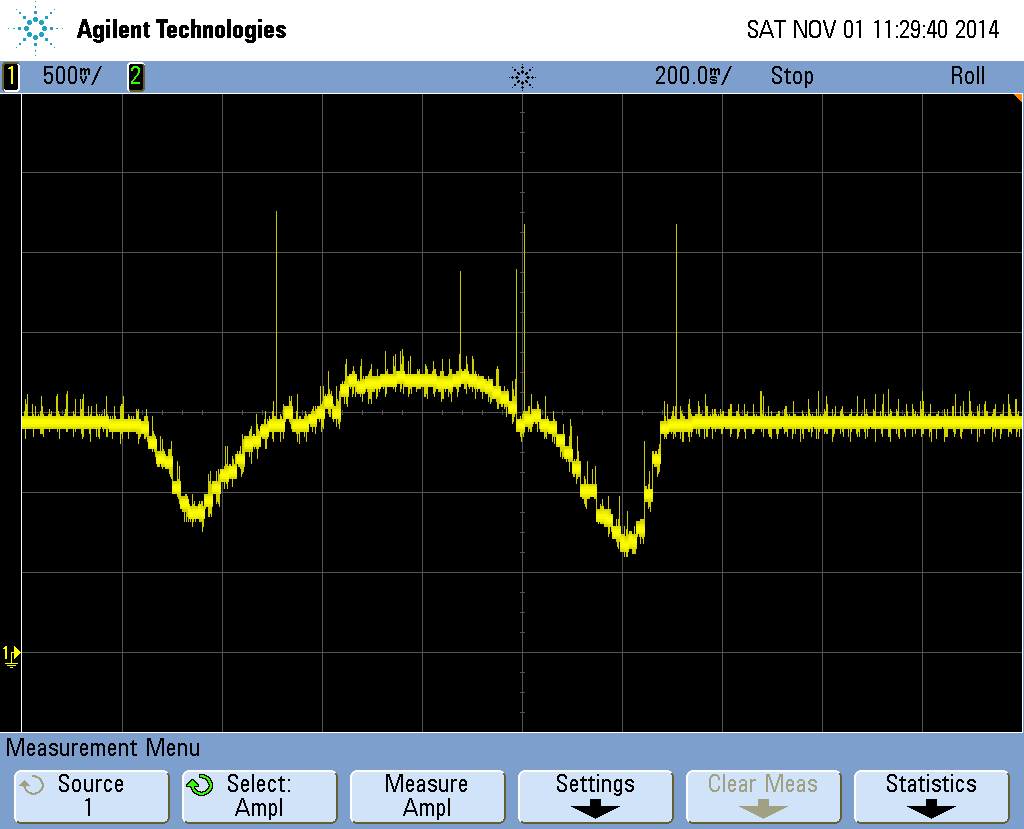
\includegraphics[width=0.4\textwidth]{fig/scope_75.png}
    \caption{Durchfahren mit Schwarzem Eimer}
    \label{fig:shift_ir_black}
\end{figure}
\begin{figure}[h!]
    \centering
    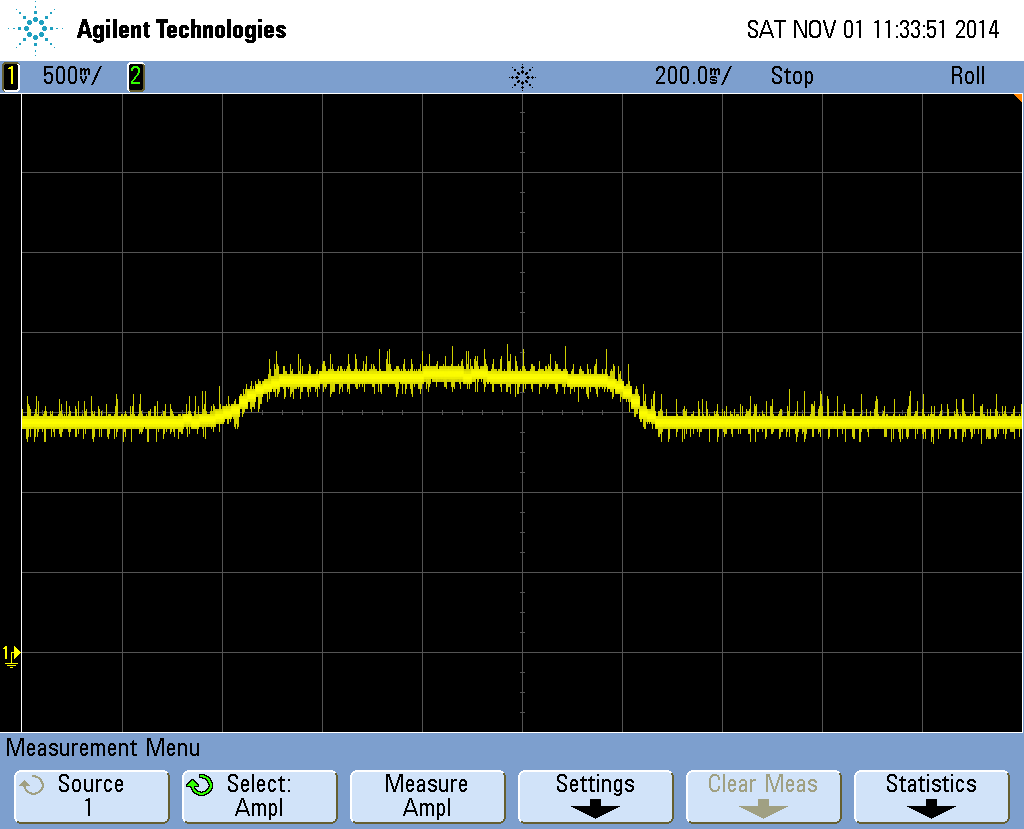
\includegraphics[width=0.4\textwidth]{fig/scope_77.png}
    \caption{Durchfahren mit Weissem Eimer}
    \label{fig:shift_ir_white}
\end{figure}

\subsubsection{Messung Scan mit Servomotor}
Als letzter Versuch wird der Sensor auf ein Servo montiert und hin und her 
gedreht. Damit wird ein Scan, wie er in einer Anwendung durchgeführt wird, 
nachgebildet. Die Dauer eines Scans beträgt 0.72 s. Der Abstand zwischen 
Eimer und Sensor beträgt 1.39 m. Die Wand hinter dem Eimer hat eine Distanz 
von 2 m zum Sensor. Auch dieser Versuch wird mit einem schwarzen und mit einem 
weissen Eimer durchgeführt. 
\begin{figure}[h!]
    \centering
    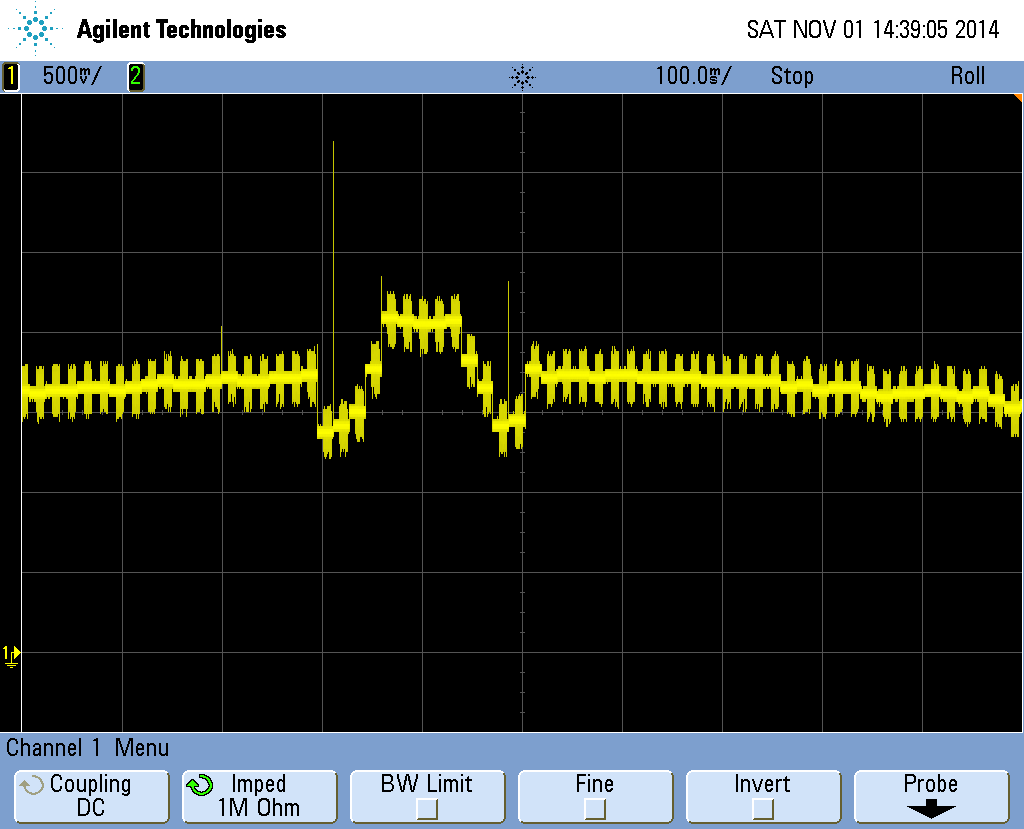
\includegraphics[width=0.4\textwidth]{fig/scope_80.png}
    \caption{Scan mit Schwarzem Eimer}
    \label{fig:scan_ir_black}
\end{figure}
\begin{figure}[h!]
    \centering
    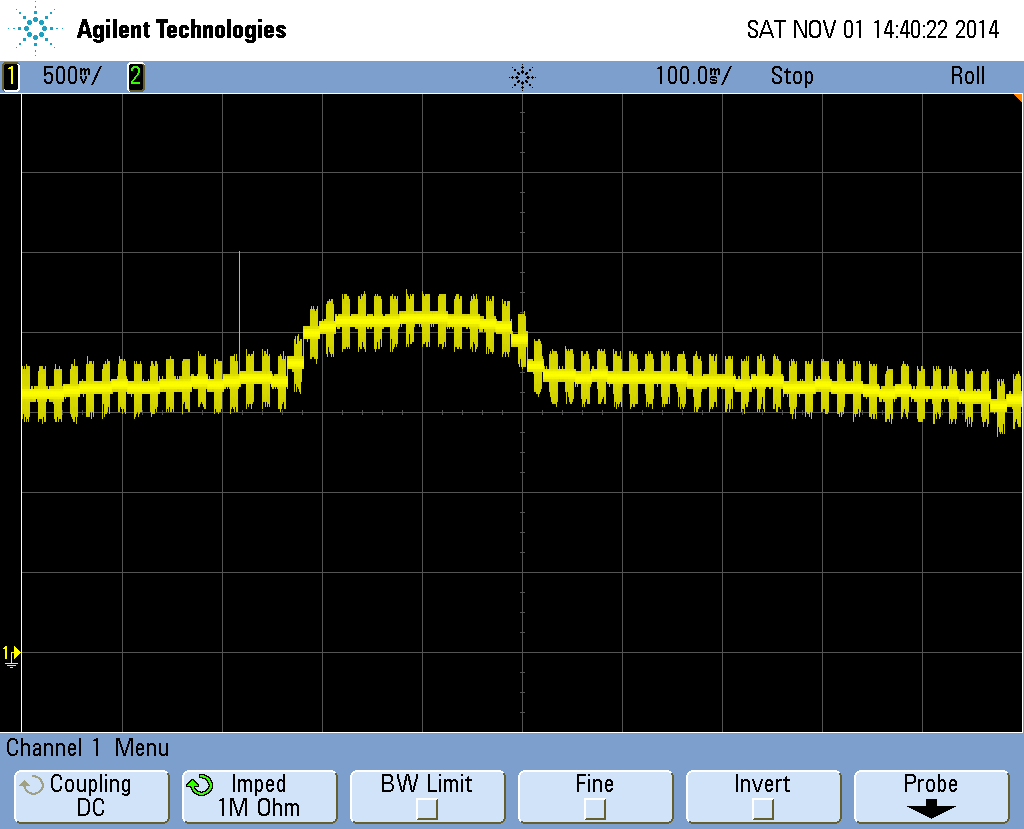
\includegraphics[width=0.4\textwidth]{fig/scope_82.png}
    \caption{Scan mit Weissem Eimer}
    \label{fig:scan_ir_white}
\end{figure}

\clearpage

\subsection{BLDC Ansteuerung}
Diese Messung wird gemeinsam mit Gruppe 32 durchgeführt. \\
